\chapter{PLUME laboratory testing}
\label{chap:labTests}

  The chapter~\ref{chap:vxd} has described the \gls{PLUME} project with the different prototypes that were built. 
  Since the version-1 of \gls{PLUME}, the detector is more complicated due to the six sensors on a module that have to be synchronised and the flex-cable which has a lot of thin metal traces to pilot and read the sensors.
  Before to perform test in real conditions at CERN or at DESY, the device has to be validated and characterised first in the lab.
  This chapter is introducing the different steps from the assembly procedure performed at Strasbourg (for the module) and Bristol (for a complete ladder), to the final tests with a radiation source, and include electrical functionality tests.

  %The \gls{PLUME} ladders are complex detectors and the last prototype was designed to optimise the material budget, by decreasing the width of the flex-cable and the metal traces.
  %Before to perform test in real conditions, the device has to be validated and characterised first in the lab.
  %This chapter is introducing the different steps from the assembly procedure performed at Strasbourg and Bristol, the electrical functionality checks to the tests with a radiation source,
 
 \minitoc
  
  %\begin{itemize}
  %  \item Describe bench
  %  \item Describe control of a sensor
  %  \item Describe output of Mi-26
  %\end{itemize}

\section{Visual inspection}

  The ladders are built in two steps. 
  Firstly, two independent modules are mounted at Strasbourg, then tested at DESY, to be then shipped at Bristol were the modules are glued together on a \gls{SiC}.
  The assembly procedure are introduced here and then the visual inspection is described.

  \subsection{Module and ladder assembly}

    \subsubsection{Module assembly}
    \label{subsec:modAssembly}

      The module assembly is performed at the IPHC by the microelectronics group and is done in three steps.
      First of all, the passive components are soldered onto a flex-cable.
      Then an epoxy layer with a thickness of $300 \mu\text{m}$ is glued under the connector side.
      This layer is used to reinforce the flex-cable on this non sensitive part due to the force applied by pulling and pushing the jumper cable.
      The module is then placed on a metal jig to insure its flatness thanks to a vacuum suction.
      The next step consists to glue the six sensors onto the flex.
      As they are thin and fragile pieces, the manipulation is done thanks to a vacuum sucker.
      Few drops of glue are dispensed on the flex and then the sensors are gently pressed one by one on top of it to be glued.
      The glue is then cured in a oven.
      The positioning of the sensors was used to be done manually, but a programmable robot is now in charge of it.
      The maximum mismatch alignment reaches $20 \mu\text{m}$. 
      The gluing procedure is definitive. 
      If a sensor is not working properly, it can't be removed and replaced by a new one because of the fragile flex-cable.
      On the worse case, a new sensor can be glued on top of it, but this procedure will increase the material budget.
      In order to avoid this situation, the sensors are probe tested at IK in Frankfort before the module assembly to select only the good ones.
      The final step consists to solder the 540 wire-bonds (a single MIMOSA-26 requires 90 wire-bonds) thanks to a semi-automatic machine.
      The wire-bonds can be protected by applying a glob top epoxy.
      It has the advantage to offer a protection against moisture ore contaminants, an electrically insulation and prohibits their movement during other manipulations. 
      Nevertheless, it increases the material budget on this area and if there is an electrical problem, the wire-bonds can't be disconnected.
      To test the module, it is transferred onto a plastic sole that has alignment pins.
      This sole is completed with a plastic cover to protect completely the module during shipping.

      %Control of absolute position about 10 $\mu\text{m}$.
      %Distance between edge of pixel of neighbouring sensors about $500 \mu\text{m}$.
      %Mismatch about $20 \mu\text{m}$.

      %The next step is to sold the wire-bonds (90 for a single Mi26) : semi-automatic machine
      %Modules are then transferred onto a plastic sole for testing and or shipping.

    \subsubsection{Ladder assembly}

    The ladder assembly is performed by the Bristol team.
    It consists to group two modules together on a spacer (\gls{SiC}) and a bate (an aluminum plate).
    The operation is done entirely by hands.
    Each module are placed on a separate jig thanks to alignment pins to ensure the positioning.
    The sensor side is facing the jig to have an access to the rear of the module for gluing.
    Then, the foam is placed on one module below the sensors, while the bate is glued below the connector with and overlaps the foam.
    The second module receives some glue on the backside before the jigs are assembled together.
    The glue is then cured for one day.
    The amount of glue needed for the assembly was studied carefully. 
    Indeed, the surface of the foam is not regular, so if not enough glue is used, the foam will not be glued on the module.
    On the other hand, using too much glue might stick the jigs together.
    When the ladder is finally ready, it is placed in an aluminum box used for shipping but also testing.
   
  \begin{figure}[!h]
    \centering
    \begin{subfigure}[t]{0.4\textwidth}
        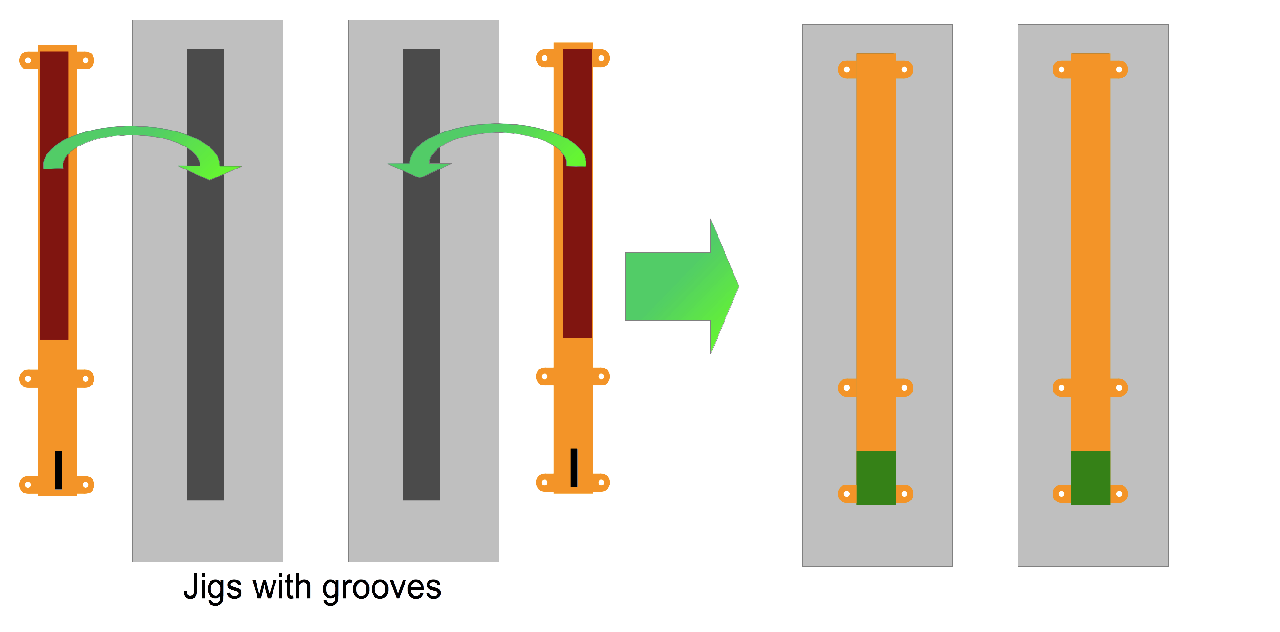
\includegraphics[width=1.3\textwidth]{Pictures/labTests/plumeLadderAssembly_step1.png}
        \caption{}
        \label{fig:ladderAssemblyStep1}
    \end{subfigure}
    \qquad
     %add desired spacing between images, e. g. ~, \quad, \qquad, \hfill etc. 
      %(or a blank line to force the subfigure onto a new line)
    \begin{subfigure}[t]{0.4\textwidth}
        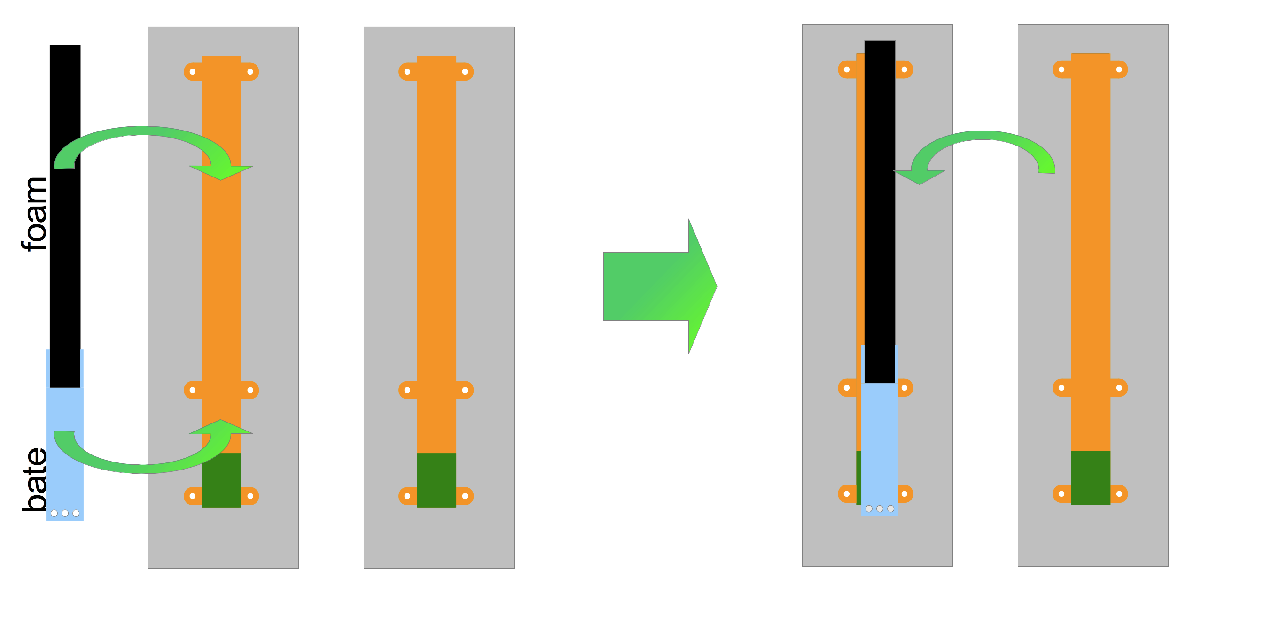
\includegraphics[width=1.3\textwidth]{Pictures/labTests/plumeLadderAssembly_step2.png}
        \caption{}
        \label{fig:ladderAssemblyStep2}
    \end{subfigure}
    \caption{Drawing of the ladder assembly. The modules are first placed on the jigs, sensors facing the grooves~\ref{fig:ladderAssemblyStep1}, then the foam and the bate are glued between the two modules~\ref{fig:ladderAssemblyStep2}.}\label{fig:ladderAssembly}
    \end{figure}    

  \subsection{Visual inspections}

  As explain in subsection~\ref{subsec:modAssembly}, the sensors positioning was performed firstly manually and later was switched to an automatic procedure.
  To tune properly the robot which is in charge of gluing the sensors on the flex-cable, the microelectronic group needs a position feedback.
  The modules are then inspected under a microscope to measure the gap between two sensors, and their position relatively to each other.
  The distance between the last pixel of a sensor to the neighboring one should be less than $500 \mu\text{m}$.
  The mismatch of the robot is about $20\mu\text{m}$. 
  The figure~\ref{fig:visAlign} is a picture taken with a microscope showing the relative position of two sensors on the bottom of the matrix for a aluminum straight module.
  %A visual inspection of the position,  as well as any problem on the matrix, as a crack, as well as a check of the wire-bonds have to be done before any electrical validation.
  The gap between the two edges is approximately $51 \mu\text{m}$. 
  
  \begin{figure}
    \centering
    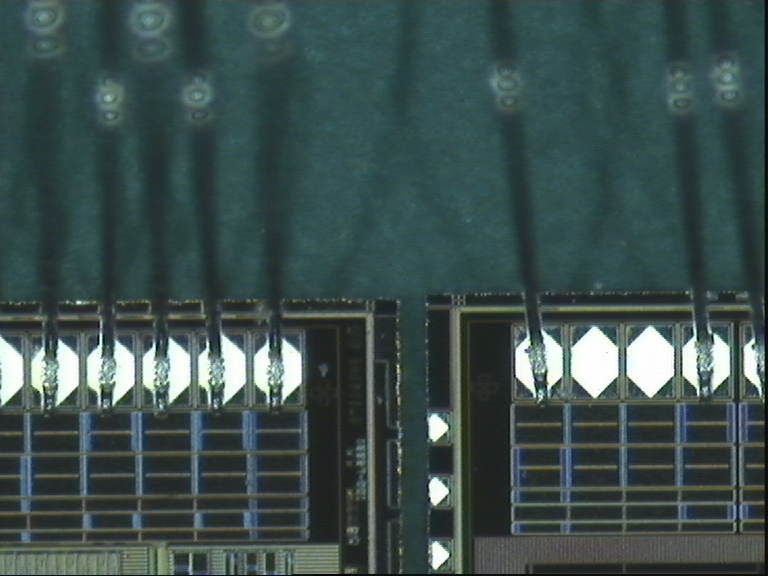
\includegraphics[width=0.6\textwidth]{Pictures/labTests/alignment_sensors.jpg}
    \caption{Visualisation of the alignment. The distance between the two edges is approximately $51 \mu\text{m}$.}
    \label{fig:visAlign}
  \end{figure}
  
  The visual inspection is also needed to check if the wire-bonds are correctly connected to the right sensor's pad, to verify that the gluing of the sensors on the flex-cable did not break the matrix and also to control that the shipping of the module between the labs (for example between Strasbourg and DESY) did not damage it.
  The module are fragile objects that have to be manipulated with care.
  Any wrong manipulation can damage severely the vital functionality.
  For example, the figure~\ref{fig:wireBondsCrashed} shows a picture taken with a microscope of wire-bonds crashed due to a falling cable on it.
  Because of the contact between some wires, the module was not working.
  Fortunately, the microcircuit group at Strasbourg was able to repair the damages and this module was operational then.
  To avoid this kind of accident to happen again, the modules were manipulated on a bench were the cables were tight and sheet of paper forbidden. 
  Therefore, the paper is able to chop off this wire.
  By using the glob-top method, the wire-bonded could have survived to a falling cable, but if the wire-bonds are not well assigned, there is no possibility to correct it.

  %\begin{itemize}
  %  \item Check positioning matrix defect (crack)
  %  \item Check wire bonds
  %  \item Check alignment
  %\end{itemize}

  \begin{figure}[!h]
    \centering
    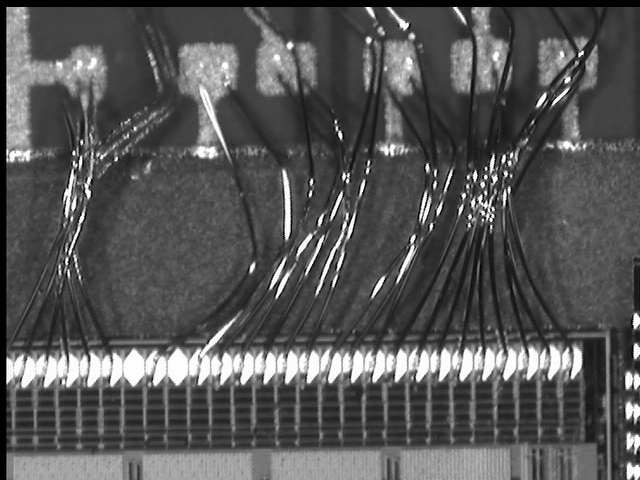
\includegraphics[width=0.6\textwidth]{Pictures/labTests/crash_bonds.jpg}
    \caption{Picture taken with a microscope showing wire-bonds crashed due to a falling cable.}
    \label{fig:wireBondsCrashed}
  \end{figure}

\section{Electrical validation}

  The electrical validation of a \gls{PLUME} module or ladder is performed in two steps.
  The first one consists to check that all the system controlling and powering the module is working. 
  Then, the module is connected and its consumption, as well as the communication are checked.

  \subsection{Auxiliary board}

  A module or a PLUME ladder is connected to the outside world thanks to a jumper cable plugged on a ZIF connector at one edge of the module.
  This jumper cable is linked to an auxiliary board which is in charge to power the sensors of the module, but also to pilot them and to transfer the data to the data acquisition system.
  This auxiliary card is connected to a power supply board which is in charge to provide the nominal voltages needed by the sensors.
  The power supply board delivers the digital and analogue voltage ($V_{DD_D}$ and $V_{DD_A}$ are set to 3.3 V thanks to two potentiometers), the $V_{CC}$ fixed to 3.3 V for the buffers, the voltage needed for the temperature measurement, a $\pm 5$ V for trigger and a power pulsing signal.
  For the lab tests to validate the module, the power pulsing is deactivated by connecting this pin to the +5 V pin of the trigger.
  The clamping voltage $V_{clp}$ used for the polarisation of the pixel has to be in the range $\left[2, 2.2\right]$ V.
  On the first version of the auxiliary board, it was provided by an external power supply, but the new version delivers the 2.1 V needed, thanks to an I2C chips or a potentiometer (the user can select which methods to use thanks to a jumper).
  The auxiliary board is also connected to a computer in charge of the sensors' slow control.
  Two RJ45 are providing the JTAG registers, as well as the start and reset signal. 
  For a complete ladder, the two modules have to be synchronised and the clock can be injected by a clock distribution board.
  One RJ45 connector is dedicated to the JTAG slow control is delivering four signals: 

  \begin{itemize}
    \item \textbf{Test Data In (TDI)}: received the serial data input feed to the test data registers or instruction register
    \item \textbf{Test Mode Select (TMS)}: controls operation of test logic (for example, by selecting the register)
    \item \textbf{Test Clock (TCK)}: uses to load test mode data from TMS pin and test data on TDI pin at the rising edge, while at the falling edge, it is used to output the test data on the TDO pin.
    \item \textbf{Test Data Out (TDO)}: the output data feed the input data of the next sensor and the last sensor sends the information back to the computer 
  \end{itemize}

  The second RJ45 connector is providing signal coming from the DAQ:
  \begin{itemize}
    \item \textbf{Clock}: clock at 80 MHz provided by the clock distribution board to synchronise two modules together
    \item \textbf{Start}: signal provided by the DAQ software to start and synchronise multiple sensors (the JTAG start works only for one sensor).
    \item \textbf{Reset}: reset the registers to default value. 
  \end{itemize}

  The principle of the connection between the auxiliary board and the different components to operate one module is depicted on the figure~\ref{fig:plumeAux}.

  Before to connect a PLUME module to the auxiliary board, the voltages have to be set and the JTAG communication has to be checked on the auxiliary card.
  Two external power supplies are delivering 8 V D.C. to the power supply board and are giving an information on the consumption of the whole system.
  The empty auxiliary board has a current consumption about 350 mA.
  Then, the $\text{V}_{CC}$, $\text{V}_{DD_d}$ and $\text{V}_{DD_a}$ should be at 3.3 V, but only the two last voltages can be adjusted thanks to two potentiometers on the power supply board.
  The $\text{V}_{clp}$ is set to 2.1 V and should not be outside the range $\left[2, 2.2\right]$ V.
  The JTAG communication is verified thanks to a probe linked to an oscilloscope.
  The observed values should be:

  \begin{description}
    \item[TDI:]
    \item[TDO:]
    \item[TMS:]
    \item[TCK:] this clock is slower (30 kHz) than the 80 MHz needed by the sensors and is only dedicated for the slow control
    \item[Reset:] by default is fixed to 1 and should change to 0 every time the reset is called by the JTAG software
    \item[Start:] 
    \item[Clock:] Independently of the method used, the 80 MHz clock has to be correctly distributed along the auxiliary card
  \end{description}

 % On one edge of the module, a ZIF connector is used to power the sensors, but also to pilot them and to transfer the data to the outside world.
 % A jumper cable is connected between the module and an auxiliary board.
 % This card is connected to a power supply board which is providing the nominal voltages needed by the module.
 % 
 % The $\text{V}_{DD_d}$ and $\text{V}_{DD_a}$, used for the buffer, are tunable thanks to two potentiometers, while $\text{V}_{CC}$, used for buffers is fixed to 3.3 V.\todo{Look for VDD and VCC}
 % The auxiliary board is also connected to a computer for the slow control.
 % Two RJ45 are in charge to provide the JTAG registers, as well as the start, the reset signal and in a case of a complete ladder an external clock.

  %First of all, the auxiliary board is connected to the power supply board which is plugged to two external power supplies, which are delivering  8 V D.C.
  %The current of the empty auxiliary board should be about 350 mA.
  %The first step is to check the different voltages on the auxiliary board.
  %The $\text{V}_{CC}$, $\text{V}_{DD_d}$ and $\text{V}_{DD_a}$ should be at 3.3 V, but only the two last voltages can be adjusted thanks to potentiometers on the power supply board.
  %The $\text{V}_{clp}$ is set to 2.1 V and should not be outside the range $\left[2, 2.2\right]$ V.
  %An I2C chips or a potentiometer are providing this voltage.
  %The auxiliary board has a section dedicated to the power pulsing, nevertheless, for the purpose of the electrical validation, the system is disconnected.

  %The clock provided to the sensors should be at 80 MHz and is transmitted to the sensors via LVDS.
  %The connections of the auxiliary board to the different component are summarised on figure~\ref{fig:plumeAux}.

  \begin{figure}[!h]
    \centering
    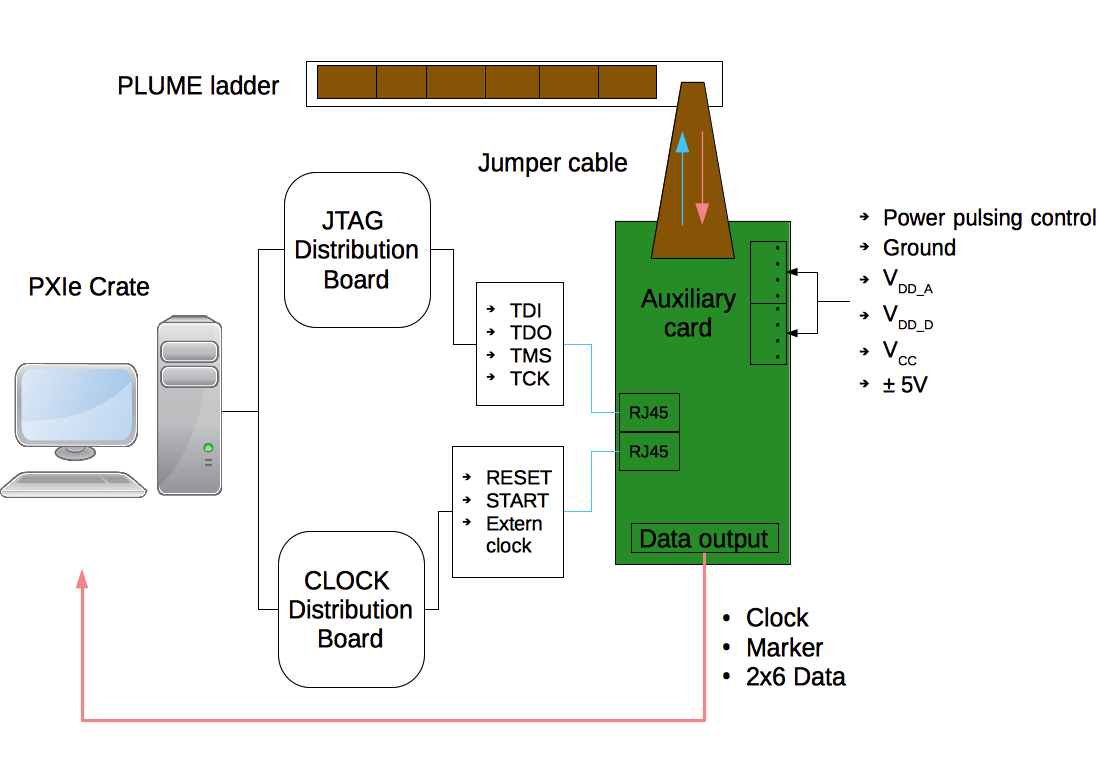
\includegraphics[width=\textwidth]{Pictures/labTests/plumeAux.png}
    \caption{Sketch of the PLUME connection.}
    \label{fig:plumeAux}
  \end{figure}


  %For the test procedure, but also for the acquisition, the PLUME module is connected to an acquisition board, via a jumper cable.
  %This board is in charge to distribute the power supplies, the control signals and the data output.
  %A power supply board is providing the $\text{V}_{dd_d}$ and $\text{V}_{dd_a}$, the $\text{V}_{CC}$ and 5 V.
  %The $\text{V}_{dd_d}$ and $\text{V}_{dd_a}$ are tunable thanks to two potentiometers, while $\text{V}_{CC}$ is fixed.

  %A PLUME module is connected to an auxiliary board via a jumper cable in order to be operated.
  %This auxiliary board is providing the power supply and the slow control to the ladder and give then an access to the sensors' output.
  %Two RJ45 inputs are providing the slow control, the reset and start signal and has the possibility to provide an external clock, used only when two modules are working together to make sure that they are synchronised.
  %A power supply board, connected to the auxiliary board, is providing the digital and analog voltage, plus 

  %An auxiliary board is in charge to power a PLUME module and to send the slow control to pilot each sensor. 
  %If only one module is tested, an oscillator is providing the 80 MHz clock.

  %Sixteen pads are used to read the response of the six sensors and the clock and marker of the sensor number 6.
  %It also has an output connection to check the response of each sensor with an oscilloscope, as well as for the acquisition.
  %It is in charge to provide the 80 MHz clock, via oscillator or via an external input. 

  %\begin{itemize}
  %  \item Generate the 80 MHz for the 6 Mi 26 by oscillator on board or by an external input.
  %  \item Bufferisation of the Digital signals sent to the chips (JTAG and control signals) and the digital signal provide by the 6 Mi26 to the DAQ in LVDS .
  %  \item Regulators for the power supply of the sensors.
  %  \item Power pulsing
  %  \item Current measurement
  %  \item test point for the DAC characterisation
  %\end{itemize}

  \subsection{Smoke test}

 % After the connections were controlled and before to connect the module to the bench, the different voltages has to be set.

  After the validation of the auxiliary board (and the power supplies switched-off), the module can be linked to it via a jumper cable.
  The voltages applied to the device have to be adjusted again due to the dissipation inside the flex-cable and the jumper cable.
  The $V_{DD_D}$, $V_{DD_A}$ and $V_{clp}$ can be measured on different pads of the ladder: three pads are closed to the connector, while the three others are at the edge of the flex-cable, as seen on the figure~\ref{fig:voltagePads}

  \begin{figure}[!h]
    \centering
    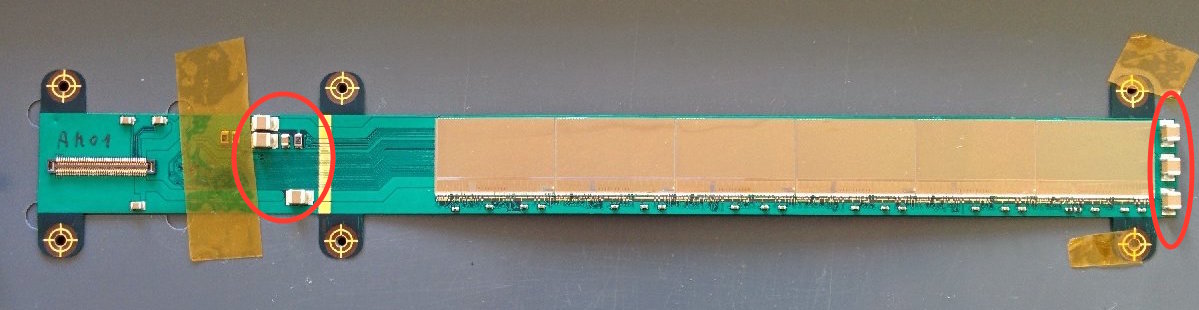
\includegraphics[width=\textwidth]{Pictures/labTests/AM01_voltagePads.jpg}
    \caption{Picture of a aluminum mirrored module with the points of measurement for $V_{DD_D}$, $V_{DD_A}$ and $V_{clp}$.}
    \label{fig:voltagePads}
  \end{figure}

  Two versions of the jumper cable, one very flexible with a high resistivity and the second one stiff with a low resistivity.
  The first cable was not used because of the high resistivity that implies an important voltage drop between the auxiliary board and the module.
  Moreover, the cable was not properly grounded.
  The second one has a low voltage drop, nevertheless, the stiffness of the cable requires a mechanical structure to hold the whole system to reduce the mechanical stress on the connector of the module, which is a sensitive part.\todo{Details of voltage drop inside the jumper cable and the flex-cable}

  The module consumption is checked at every JTAG steps to make sure that no short-circuit occurs.
  Right after powering-on the system, the six sensors are starting in a random state and the consumption at this stage can not point out any electrical problem.
  After the reset of the registers, the total consumption should be around 33 mA.
  Then, the registers are loaded and the consumption should be around 750 mA and read-back by the JTAG software.
  If at the reading step no error was discovered, the sensors can be operated and their consumption should be around 1300 mA.

  %Before to present the next step to control the JTAG communication of every sensor, let's introduce the MIMOSA-26 output.

  %\subsection{Mimosa-26 output}

  An inspection of the output with an oscilloscope is performed to check the slow control and to estimate the response of the sensor.
  For the normal mode data format with SUZE enable, the output data of the last frame is sparsified and transmitted during the acquisition of the current one.
  The information provided by the MIMOSA-26 is contained in four output lines.
  The first output line corresponds to the \textit{clock} which is always running even if the data transmission is finished. 
  Its rate depends on the clock rate register. 
  For the normal output mode, it is 80 MHz.
  The second output line is the \textit{marker}, which is available in all mode.
  It is set during four clock's rising edge cycle and might be used to detect the beginning of the data transmission.
  Then, the two last output lines are dedicated to the data.
  They contain multiple information.
  First of all, the beginning and the ending of the data transmission is determined by the \textit{header} and \textit{trailer}.
  They can be used to detect a loss of synchronisation.
  They corresponds to $2 \times 16$ bits (\textit{header0-header1} and \textit{trailer0-trailer1}) and are totally configurable through the JTAG software.
  The \textit{header} is followed by the \textit{frame counter} which corresponds to the number of frame since the chip was reset. 
  The information is separated into two words (\textit{FrameCounter0} corresponding to the least significant bit and \textit{FrameCounter1} corresponding to the most significant bit).
  Then, the \textit{data length} gives the number of 16 bits words of the useful data. 
  The useful data is split into \textit{states/line}, which contains the address of the line which has a hit and an overflow flag, followed by the \textit{state} giving the number of consecutive hit and the address of the first column.
  Finally, the \textit{trailer} is ending the data transmission followed by 32 bits of zero.
  The figure~\ref{fig:mi26Output} is a picture of an oscilloscope output of a MIMOSA-26 data output. From the top to the bottom, it shows the 80 MHz \textit{clock}, the four clock's cycle \textit{marker}, the \textit{data0} and \textit{data1} with the \textit{header} and the \textit{frame counter}.
  More information about the MIMOSA-26 can be found here\todo{Reference to MI-26 user manual}.

  \begin{figure}[h]
    \centering
    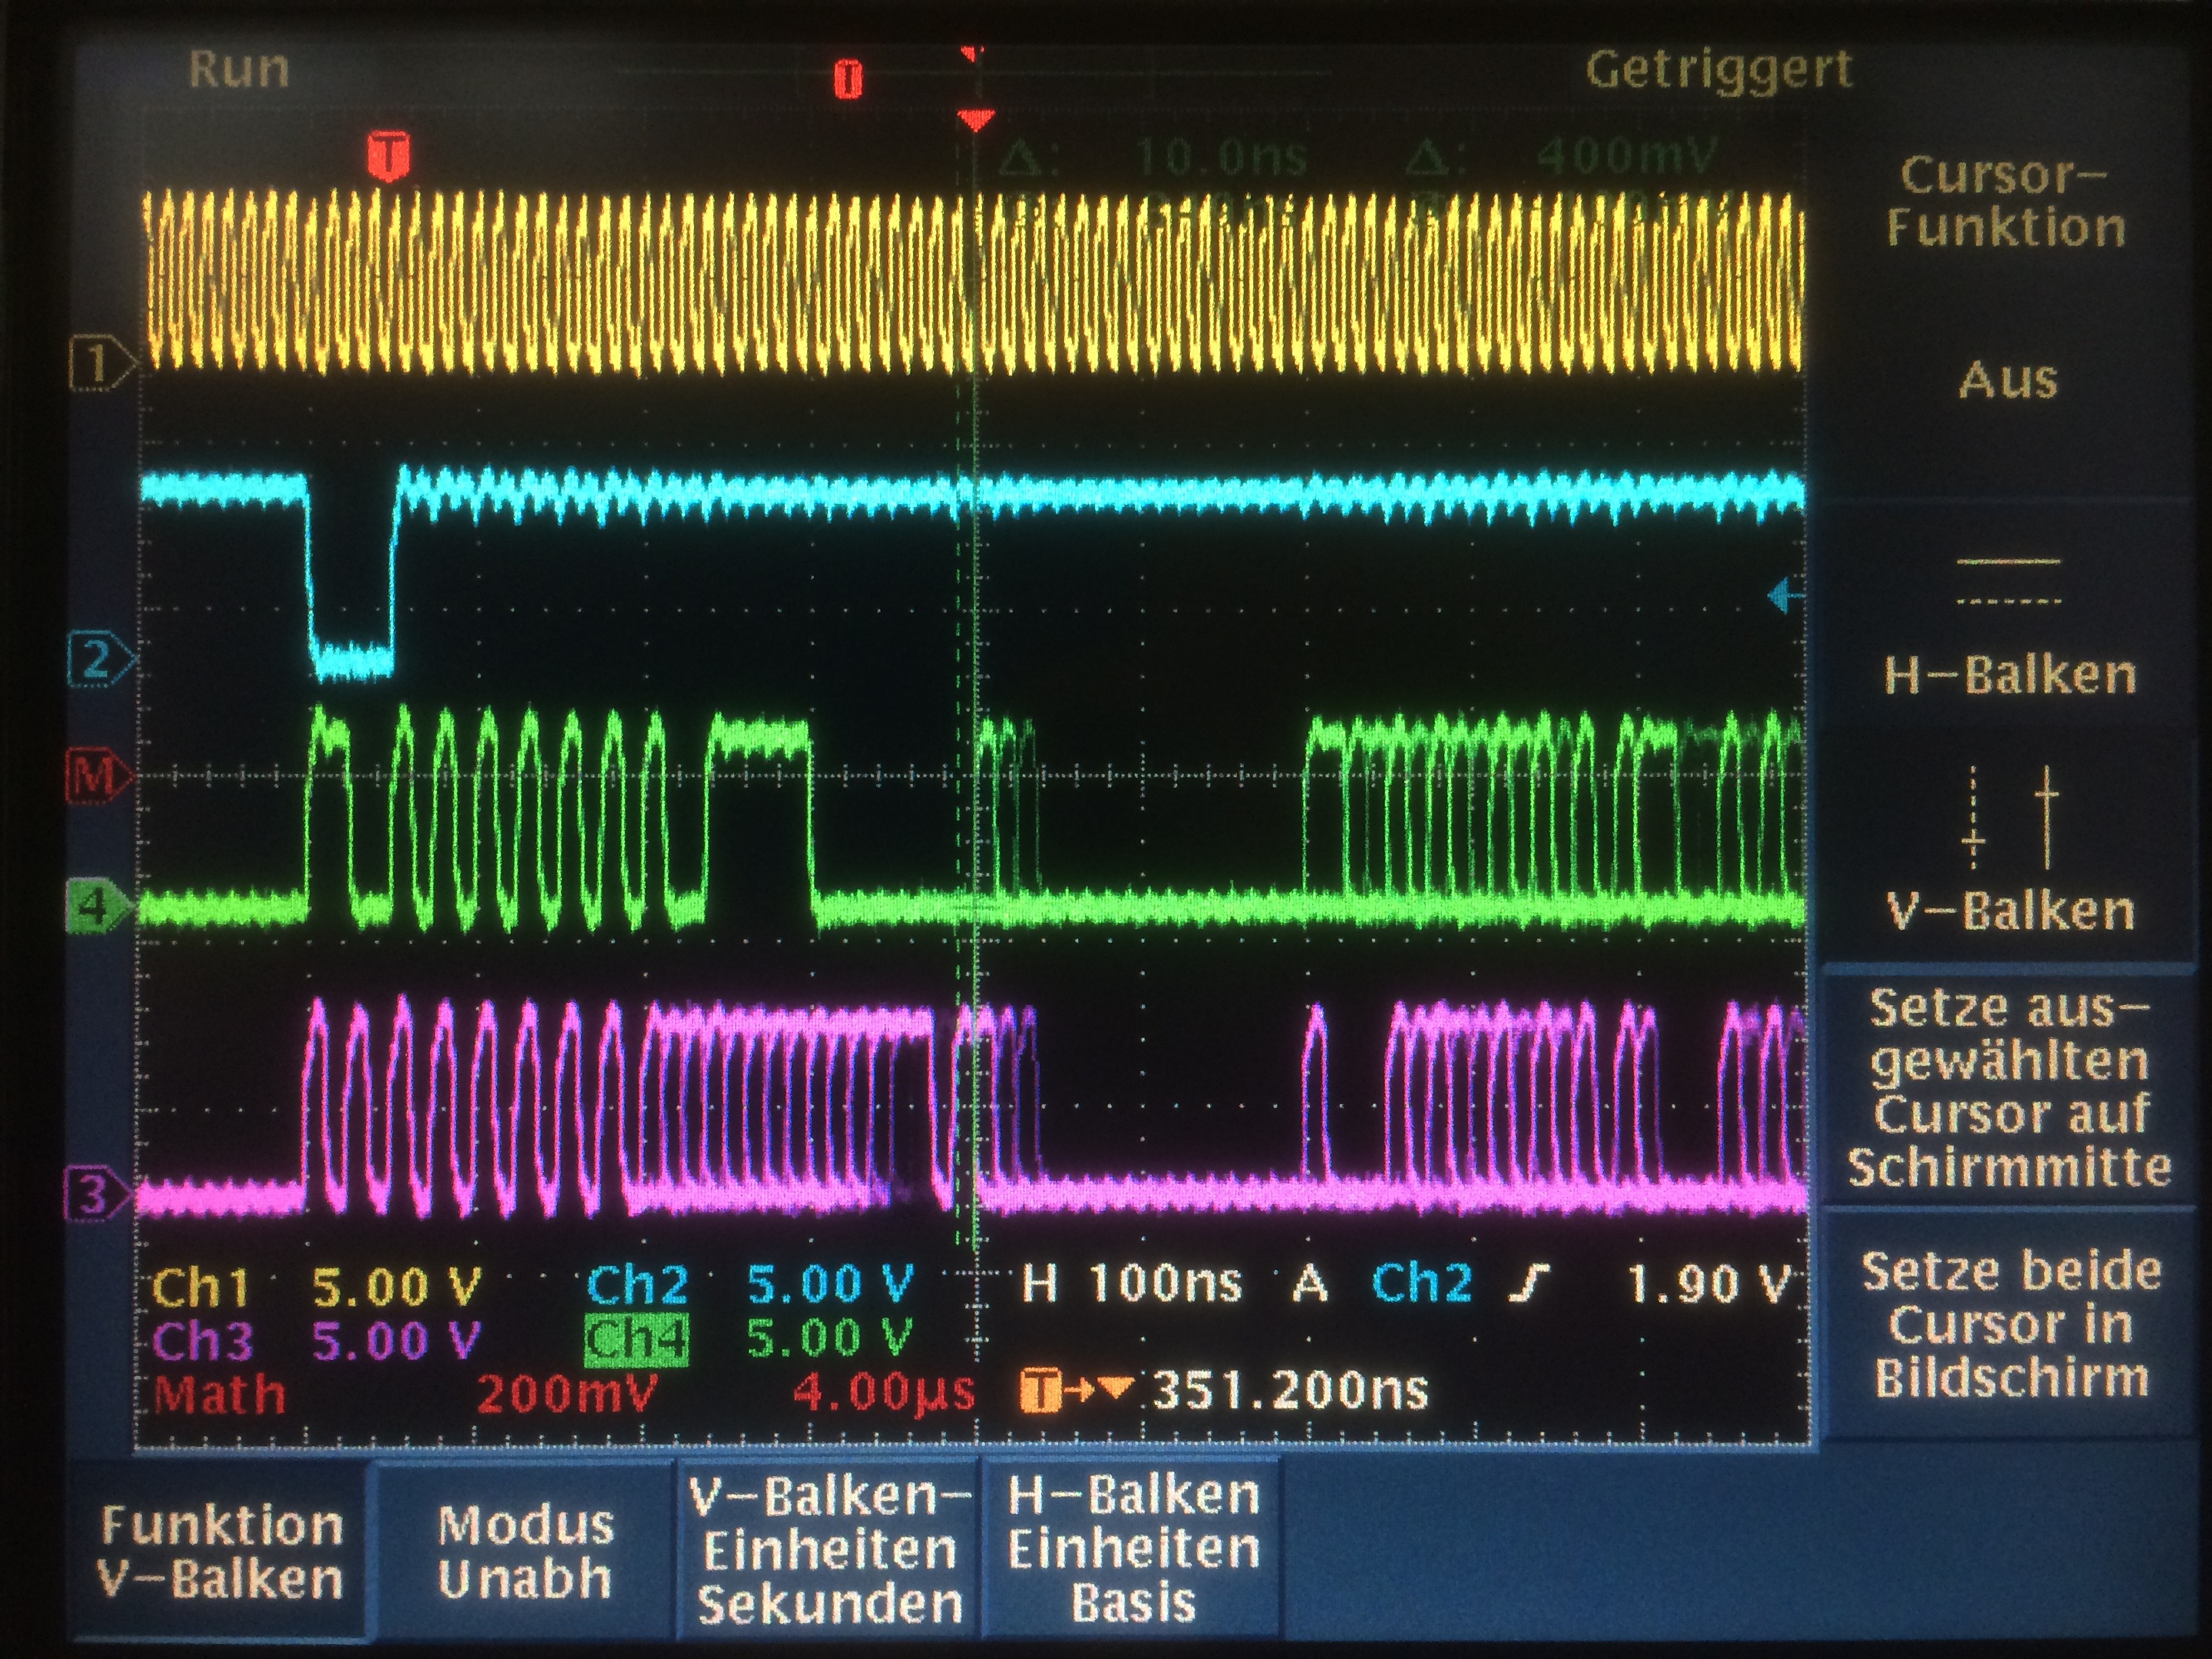
\includegraphics[width=0.8\textwidth]{Pictures/labTests/mi26_output}
    \caption{MIMOSA-26 output from oscilloscope. The top yellow line corresponds to the clock, the blue line below to the marker (which last 4 clock cycles), and the green and purple line are the data output containing the hit information}
    \label{fig:mi26Output}
  \end{figure}

  \subsection{JTAG communication}

  After adjusting the voltages and looking for any short-circuits, the next step is to control the JTAG communication for every sensor.
  As in the PLUME module, all the sensors are synchronised, only the \textit{clock} and \textit{marker} from one sensor is read back.
  On the oscilloscope, the trigger is set on the \textit{marker}.  
  The sensors are configured in the normal mode data format (80 MHz with zero suppression output) and the output is checked in three steps.
  First of all, the sensor is reset, the register are loaded and read back and then the start signal is sent. 
  Through the JTAG software, the \textit{header} and \textit{trailer} are modified several time and are checked thanks to the oscilloscope.
  Then, the discriminators response is visualised, specifically to find pixels stuck in an opened position (always sending data).
  The number of defective pixels and their position is then estimated.
  After that, an estimation of the threshold discriminator values to get few hits is determined and the response is then checked.
  Nevertheless, using light to estimate the response of the sensor can impact the pixels' baseline and modify the normal behavior of the matrix.
  For example, instead of sending more information, the pixels are less responsive.
  Thus, using a radiation source is a better solution.

\section{Noise measurements}

  In the chapter~\ref{chap:vxd}, the principle of the \gls{CMOS} sensors was described and the noise of this technology was discussed.
  As a reminder, the two noises contribution are the \acrfull{TN} and the \acrfull{FPN}.
  The \gls{FPN} is determined as an offset to subtract from the pixel response to reduce its non-uniformity response, while the \gls{TN} is coming from the contribution of different noises during the reset, the integration and the readout of the pixel.
  This noises have to be measured in the lab in order to find the optimum configuration to detect physics signal and reduce the noise impact on the measurement.

  \subsection{Characterisation bench}

  The noise is estimated thanks to a bench of characterisation composed of a National Instrument PXIe crate equipped with a 6562 digital card, two power supplies, a power distribution board, an auxiliary and a JTAG card, as well as the module to test.
  The procedure described here is applied to a single MIMOSA-26, or a PLUME module, as well as a MIMOSA-28 sensor.
  Nevertheless, the data acquisition software used during the characterisation is slightly different, depending on the sensor technology.
  The four output data are connected from the pins on the auxiliary board to the digital card thanks to a National Instrument spider cable.
  Firstly, a test pattern, which loads automatically a JTAG file for this test, is done to read the \textit{header} and \textit{trailer} during several frames with a determined data length.
  It has been observed that the \textit{clock} output cable has to be eighty centimeters longer than the three other cables to ensure the synchronisation on the rising edge.
  If this is not done or if one of the cable has a wrong polarity, the software is not able to read the \textit{header} and \textit{trailer}.

  Then, the sensors are configured in the discriminator output mode.
  The zero suppression mode is bypassed, pixels and discriminators are in normal mode (whole matrix read in $115\mu\text{s}$), but the readout frequency is lower (10 MHz) via 2 LVDS output pads.
  The control of the discriminators is divided into four sub-matrices, each containing 288 columns.
  Thus, for one sub-matrix a threshold value in DAC units in the JTAG software is driving all the discriminators, depending on a baseline value.
  For one line, usually one located in the middle of the matrix, its baseline response is studied to find the "middle-points" by looking for the threshold of each sub-matrix, in which the discriminators are reaching an half activation.
  When this "middle-points" are determined, the homogeneity of the matrix is checked, as shown on the figure~\ref{fig:homogeneityMi26}.
  
  \begin{figure}[!h]
    %\centering
    \missingfigure{Homogeneity of the Mi26 matrix when the discriminators are 50 \% activated}
    \caption{Matrix response for the discriminators half activated.}
    \label{fig:homogeneityMi26}
  \end{figure}
  
  Due to the structure of the sensor, the homogeneity is not perfect and some dispersions in the discriminator response are observed between the beginning and the end of a sub-matrix.
  Moreover, to reduce this dispersion, the reference baseline and the clamping voltage have to be adjusted.
  Before to start the threshold scan, the thresholds are set to the lowest and highest value in order to look for defect pixels.
  On the one hand, few pixels can be always activated even if the discriminators were closed.
  The figure~\ref{fig:openPixel} depicts the matrix output for all the discriminators closed.
  Therefore, a line is always activated, as well as few pixels in a column and they are increasing the fake hit rate of the matrix.
  A solution exists to disconnect some discriminators in order to reduce the noise of defect columns thanks to the JTAG program, nevertheless, no solution during the sensor programming exists to remove the defect lines.
  On the other hand, few pixels can be always deactivated even if the discriminators are completely opened, thus, they are not able to detect any physics signal.
  This behavior is represented on the figure~\ref{fig:closePixel} and no solution exists to make them working properly.
   
  \begin{figure}[!h]
    \centering
    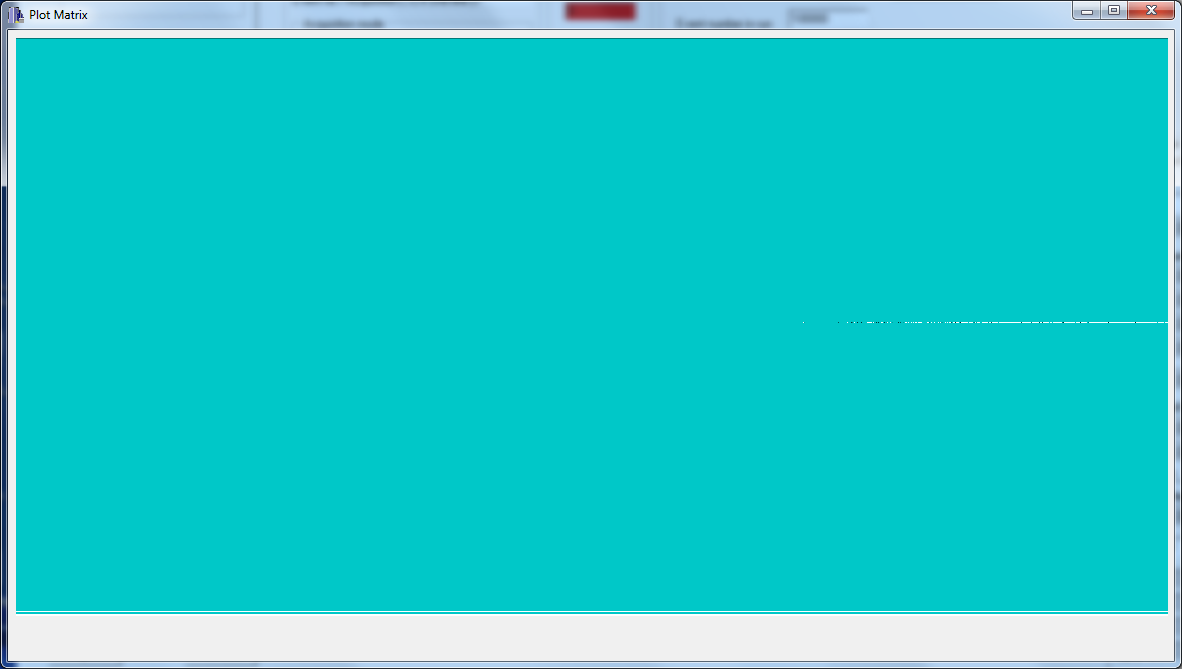
\includegraphics[width=\textwidth]{Pictures/labTests/th0.png}
    \caption{Matrix response in discriminator mode, where all the discriminators are opened. On the right of the matrix, one line is not working correctly and some pixels are never activated}
    \label{fig:openPixel}
  \end{figure}
   
  \begin{figure}[!h]
    \centering
    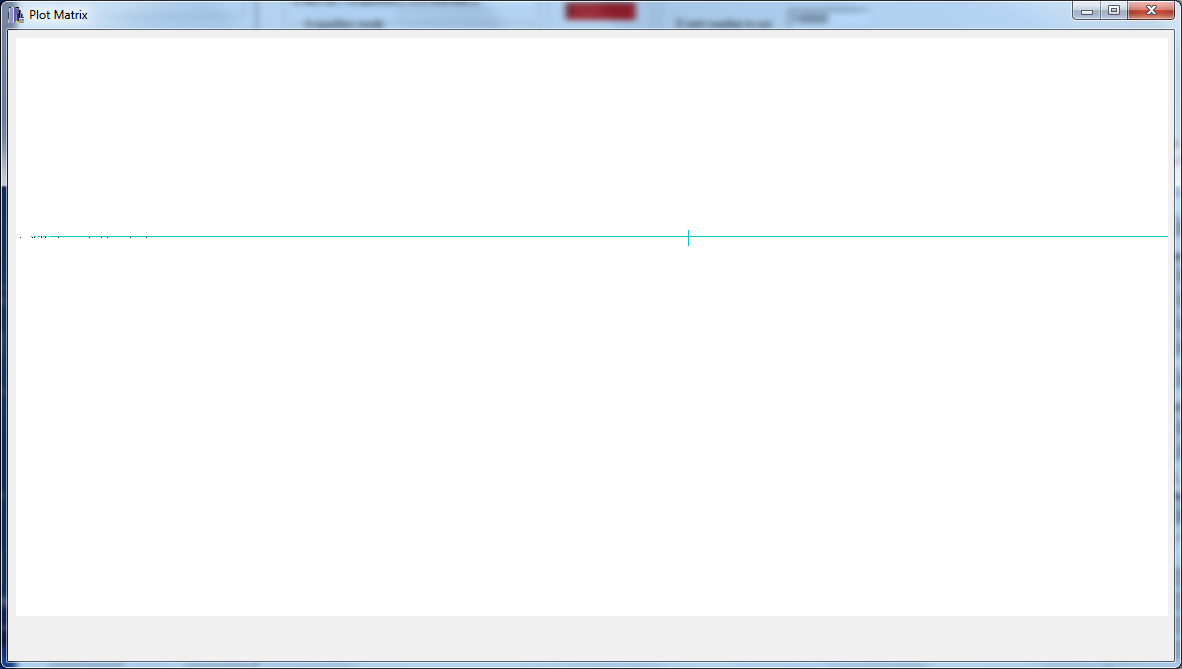
\includegraphics[width=\textwidth]{Pictures/labTests/th255.png}
    \caption{Matrix response in discriminator mode, where all the discriminators are closed. One line of pixels is always activated, as well as few pixels in the same column. This will increase the fake hit rate of the sensor.}
    \label{fig:closePixel}
  \end{figure}

  \subsection{Threshold scan}

  To measure the noise, a threshold scan is perform around the "middle-point" found before.
  For each step, the data acquisition software records the response of each discriminators, in order to calculate the noise, the offset and the dispersion.
  Usually, 29 runs with 500 to 1000 events are stored.
  They are two different ways to measure the noise. 
  The first one consists to inject a reference voltage in the discriminators, while the matrix output is disconnected.
  Only the noise contribution coming from the discriminators is thus determined.
  The second method does not use an external reference voltage, but rather the response of the pixel matrix to characterise the noise of the whole system.

  The next step consists to build a configuration file containing the DAC values of each sub-matrix for each threshold with the corresponding value in millivolts.
  %After completing the threshold scan, a configuration file, which contains the DAC values of each sub-matrix for each threshold with the corresponding value in millivolts is created.
  Afterward, this file is analysed and converted to create an output file containing a hit average picture of each sub-matrix for each step.
  Then a macro based on C++ and ROOT is reading this picture to plot the transfer function, as the one represented on figure~\ref{fig:transfer}, which shows the response of the 288 discriminators for a sub-matrix, as a function the threshold applied in millivolts.
  From this S-curve, the dispersion, as well as the offset and the noise are measured.
  Two plots are summarising this information, as shown on figure~\ref{fig:TN&FPN}.
  
  \begin{figure}
    \centering
    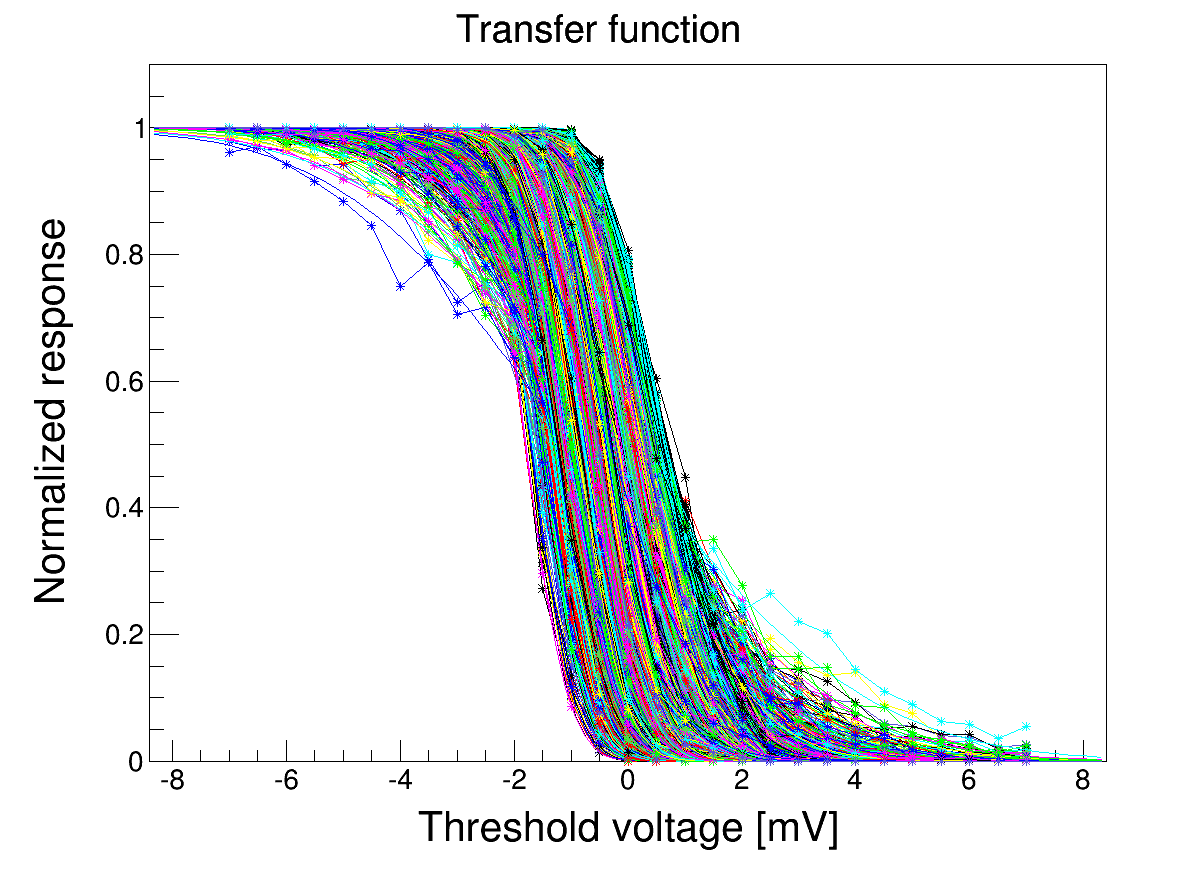
\includegraphics[width=0.6\textwidth]{Pictures/labTests/transfer_B.png}
    \caption{Pixels response of a threshold scan around the middle-point of discriminators for a sub-matrix.}
    \label{fig:transfer}
  \end{figure}

  \begin{figure}
    \centering
    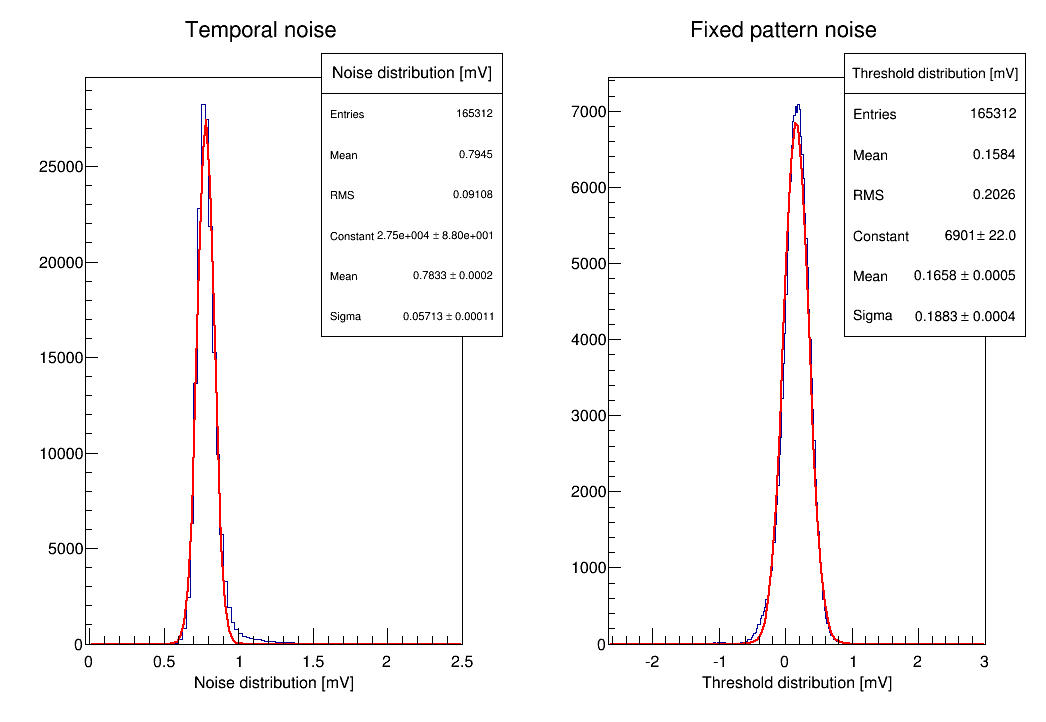
\includegraphics[width=0.8\textwidth]{Pictures/labTests/noise_A.png}
    \caption{TN and FPN}
    \label{fig:TN&FPN}
  \end{figure}

  The one on the left represents the temporal noise, while the right one represents the fixed pattern noise.
  The offset corresponds to the RMS of the fixed pattern noise, the dispersion is the ... of ... and the noise ...
  To estimate the discriminator thresholds of each sub-matrix for a given \gls{SNR}, the total noise is determined as:
  
  \begin{equation}
    \text{Total noise} = \sqrt{<TN>^2 + <FPN>^2}
  \end{equation}

  For a given S/N cut $\sigma$, the thresholds are determined by:

  \begin{equation}
    \text{Threshold (mV)} = \text{Total Noise} \times \sigma + \text{offset}
  \end{equation}

  This is converted into the DAC values by taking into account the DAC offset and the DAC slope, which is assumed to be 0.25 mV:
  
  \begin{equation}
    \text{Threshold (DAC)} = \frac{\text{Threshold (mV)} - \text{DAC}_{offset}}{\text{DAC}_{slope}}
  \end{equation}

  \subsection{Measurement of the fake hit rate}

  Once the thresholds are defined for the different cuts, the fake hit rate of the matrix, as well as the detection homogeneity is determined.
  A quick step consists to use the DAQ software and acquire ten-thousands events in the dark. 
  The fake hit rate per event per pixel is then determined as:

  \begin{equation}
    \text{F.H.R} = \frac{\text{Number of hits}}{\text{Number of events} \times \text{Number of pixels}} 
  \end{equation}
  
  The figure~\ref{fig:darkEvents} is representing the accumulation in the dark of ten thousands events for a threshold five times bigger than the noise.
  The measured fake hit rate was below $10^{-4}$ hits/pixel/events.

   \begin{figure}[!h]
    \centering
    
\includegraphics[width=0.6\textwidth]{Pictures/labTests/8sigma_10kEvents_noSource}
    \caption{Accumulation of 10k events at a thresholds of 5 times the noise acquired in the dark.}
    \label{fig:darkEvents}
  \end{figure}

  Then an iron 55 source is used to control the homogeneity of the thresholds determined before.
  The figure~\ref{fig:fe55} represents the accumulation of ten thousand events for a threshold five time bigger than the noise with a iron source on top of the sensor.
  
  \begin{figure}[!h]
    \centering
    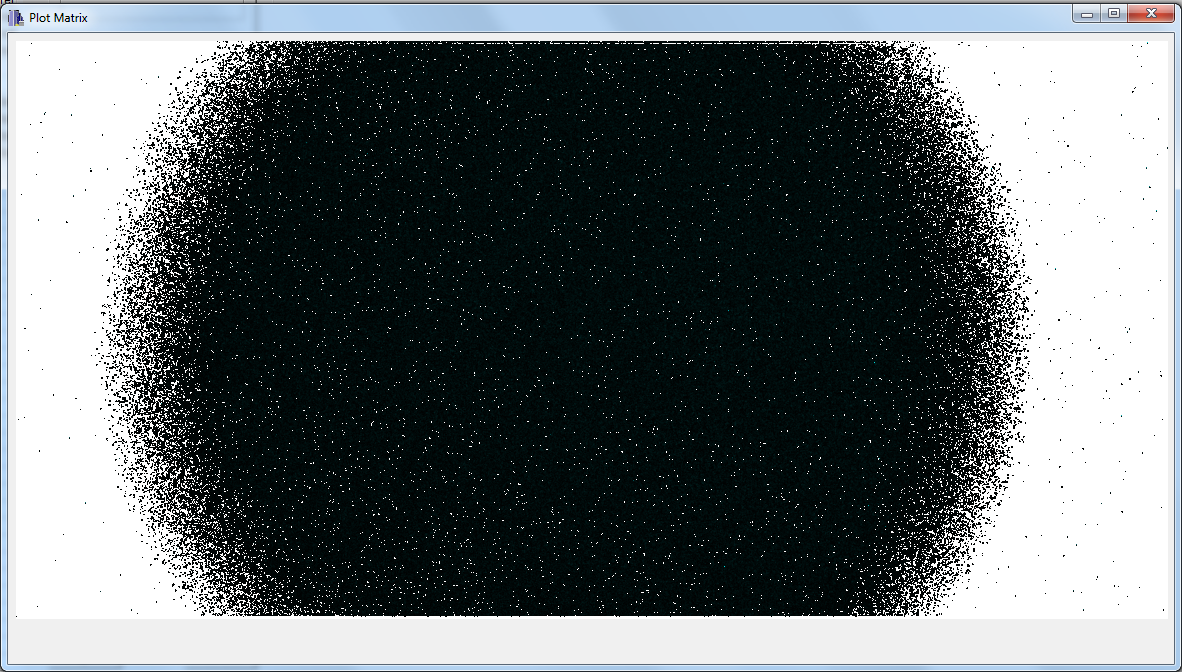
\includegraphics[width=0.6\textwidth]{Pictures/labTests/10kEvents_Fe55_cut5sigma.png}
    \caption{Accumulation of 10k events at a thresholds of 5 times the noise with Fe55 radiation source.}
    \label{fig:fe55}
  \end{figure}

  Finally, in order to validate the sensor, the acquisition system used during the test beam is used to calculated more accurately the fake hit rate.\todo{detail the DAQ}
  The auxiliary board is connected to a  Flex RIO board instead of the digital card.
  The test beam DAQ software developed by the IPHC is using LabVIEW interface, which gives the number of events acquired, the \textit{header}, the \textit{trailer} and the \textit{frame counter} of the sensor.
  A second software is used to store the data into three files: a parameter file containing the run number, the event number, a binary file containing the data and an index file.
  Two acquisition modes are available. 
  The first one, used in test beam, acquires data only when a trigger is sent.
  The second one, stores all frames regardless there is a trigger or not. 
  This acquisition is the one used in the lab, as only the noise of the sensor is measured.
   
  Several runs containing each one million events are acquired for different thresholds. 
  The data stored are analysed with a software developed by the IPHC and is called \gls{TAF}.
  It is based on C++ and the ROOT framework.
  The software reads the information of the hit pixels, reconstructs the clusters of hit pixels and in the case of a test beam is able to reconstruct tracks from the hit information.

  A method is in charge to determine the fake hit rate with respect to the number of pixels hit per event.
  From the distribution shown on the figure~\ref{fig:pixel/event}, which represents the number of pixels fired per event, the average fake hit rate is calculated as the mean of this distribution divided by the total number of pixel contained in the matrix.
    \begin{figure}
    %\centering
    \missingfigure{Number of pixels per event}
    \caption{Distribution of the number of pixel fired per event.}
    \label{fig:pixel/event}
  \end{figure}
  The error on the measurement is then the root mean squared of the distribution divided by the number of entries and the number of pixel inside the matrix.
  This calculation is done for different thresholds and the figure~\ref{fig:FHR} represents the average fake hit rate per pixel per event as a function of the threshold for one sensor of an aluminum module.
  The results are matching the expected behavior for a standalone MIMOSA-26 sensor as shown in figure~\ref{fig:mi26Perf}.

  \begin{figure}
    \centering
    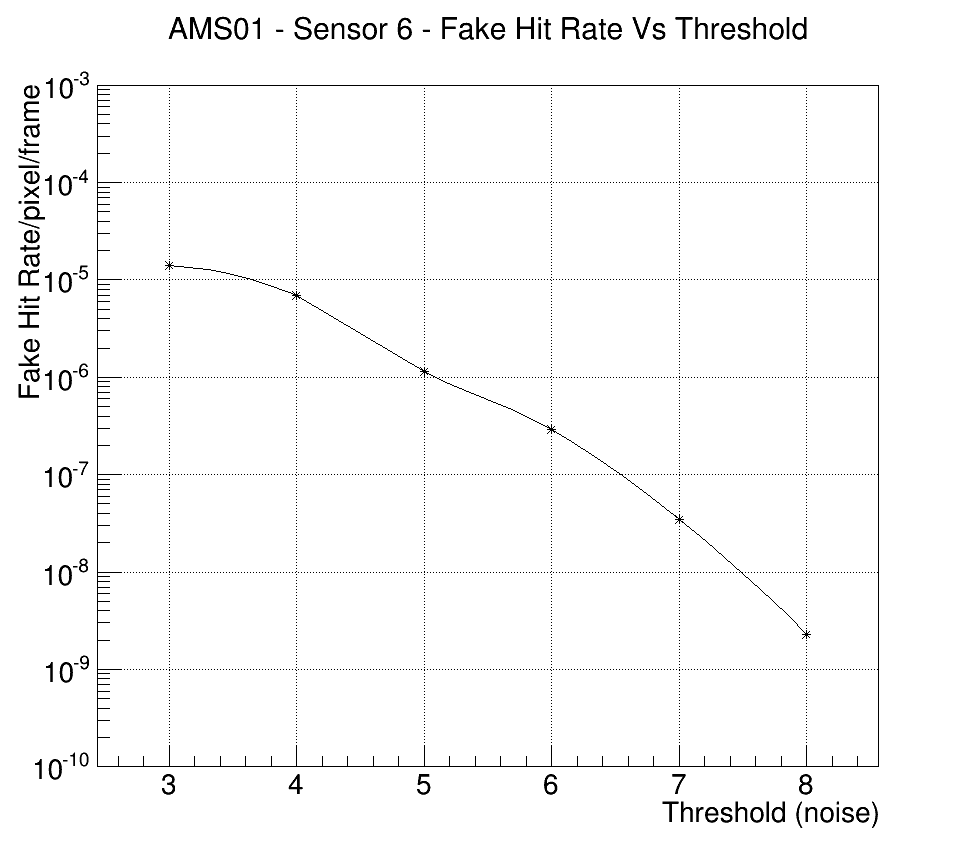
\includegraphics[width=0.7\textwidth]{Pictures/labTests/fake_sensor6.png}
    \caption{Distribution of the fake hit rate per pixel.}
    \label{fig:FHR}
  \end{figure}



\section{Cluster}

  

  \begin{figure}
    %\centering
    \missingfigure{Cluster shape}
  \end{figure}
